\documentclass[11pt]{beamer}
\usepackage{amsmath}
\usepackage{amsfonts}
\usepackage{amsthm}
\usepackage{graphicx}



\usetheme{Dresden}
\usecolortheme{seahorse}


%%theorems
\theoremstyle{plain}
\newtheorem{thm}{Theorem}[section]
\newtheorem{lem}[thm]{Lemma}

\theoremstyle{definition}
\newtheorem{defn}[thm]{Definition}
\newtheorem{prob}[thm]{Problem}


\theoremstyle{remark}
\newtheorem{rmk}[thm]{Remark}
\newtheorem{ex}[thm]{Example}

%%definitions
\newcommand{\of}[1]{\!\left(#1\right)}


\newcommand{\domain}{\Omega}
\newcommand{\boundary}{\Gamma}
\newcommand{\flow}{\vec v}
\newcommand{\refeq}[1]{(\ref{eq:#1})}

\title{\textbf{The Trace Finite Element Method for PDEs on Surfaces}}
\author{T. Jawecki, M. Wess}
\date{\today}
\begin{document}
\frame{\titlepage}

\begin{frame}
	\frametitle{Table of Contents}
	\tableofcontents
\end{frame}

%%%%%%%%%%%%%%section1
\section{Derivation of the model problem}
\begin{frame}
    \frametitle{General setting}
    \begin{columns}[T]
    	\begin{column}{0.5\textwidth}
			\begin{figure}[p]
				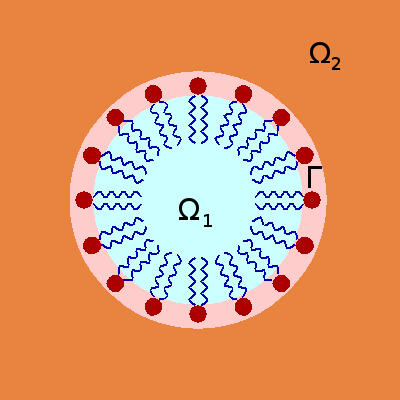
\includegraphics[width=0.7\textwidth]{surfactant3.png}
			\end{figure}
		\end{column}
		\begin{column}{0.5\textwidth}
			\begin{itemize}[<+->]
				\item{two fluids $\domain_1,\domain_2$ contained in an open domain, seperated by $\boundary$}
				\item{given velocity field $\flow$}
				\item{concentration $c$ of surfactant agent on $\boundary$}
			\end{itemize}
		\end{column}
	\end{columns}
	\begin{prob}
		For given initial data $c_0$, model the evolution of $c$.
	\end{prob}
\end{frame}
\begin{frame}
	\frametitle{Surface gradient and divergence}
		\begin{itemize}[<+->]
			\item{$C^2$-hypersurface $\boundary\subseteq\mathbb{R}^d$, outward normal $\vec n_\boundary$}
			\item{$C^1$-functions $f:\boundary\to\mathbb{R}$, $\vec g:\boundary\to\mathbb{R}^d$}
		\end{itemize}
	\only<3->{	
	\begin{defn}
		\begin{align*}
			\nabla_\boundary f&:=P\nabla f:=\left(I-\vec n_\boundary \vec n_\boundary^T\right)\!\nabla f\\
			\textrm{div}_\boundary \vec g&:=\nabla_\boundary\cdot \vec g:=\sum_{i=1}^d\vec e_i\sum_{j=1}^dp_{ij}\frac{\partial g_i}{\partial x_j}
		\end{align*}
	\end{defn}}
\end{frame}




\begin{frame}
    \frametitle{Reynolds transport theorem on an interface}

	\begin{thm}[Reynold's transport theorem on an interface]
	The rate of change for a smooth function $f(x,t)$ on $W\of{t}\subseteq \boundary$ with a given velocity field $\vec v$ can be described by
		\begin{equation}
			\frac{d}{dt}\int_{W\of{t}}f\of{x,t}ds=\int_{W\of{t}}\dot f\of{x,t}+f\of{x,t}\mathrm{div}_\boundary\of{\vec v}ds
		\end{equation}
		with the material derivative $\dot f$ defined as
		\begin{equation}
		\dot f:=\frac{\partial f}{\partial t}+\vec v\cdot\nabla f
		\end{equation}
	\end{thm}
\end{frame}

\begin{frame}
	\frametitle{Conservation of mass}
	\begin{itemize}
		\item<1->{source function $f$}
		\item<2->{velocity $\vec q$\only<4->{$:=-\alpha\nabla_\boundary c$}}
	\end{itemize}
	\begin{align*}
		\uncover<3->{
			\frac{d}{dt}\int_{W\of{t}}c\,ds
		}
		\uncover<3->{
			&=-\int_{\partial W\of{t}}\vec q\cdot n_W \,d\tilde s+\int_{W\of{t}}f\,ds\\
		}
		\uncover<5->{
			&=\int_{W\of{t}}\mathrm{div}_\boundary\of{\alpha\nabla_\boundary c}ds+\int_{W\of{t}}f\,ds\\
		}	
		\uncover<6->{
			&=\int_{W\of{t}}\dot c+c\mathrm{div}_\boundary\of{\vec v}ds\\		
		}
		\uncover<6->{
			&=\int_{W\of{t}}\frac{\partial c}{\partial t}+\vec v\cdot\nabla c +c\mathrm{div}_\boundary\of{\vec v}ds		
		}
	\end{align*}
\end{frame}


\begin{frame}{Model equation in strong form}
	\only<1-5>{since $W\of{t}$ was arbitrary and we assume $\boundary$ to be stationary:}
	\only<6>{
	for a given (tangential) velocity field $\vec v$, a source function $f$ and initial data $c_0$ find $c$ such that
	}
	\only<2-4>{
	\begin{equation}
		\frac{\partial c}{\partial t}+\vec v\cdot \nabla c + c\, \mathrm{div}_\boundary	\of{\vec v}-\mathrm{div}_\boundary\of{\alpha\nabla_\boundary c}=f.
	\end{equation}
	}
	\only<5->{
	\begin{equation}
		\frac{\partial c}{\partial t}+\mathrm{div}_\boundary\of{c\vec v}-\mathrm{div}_\boundary\of{\alpha\nabla_\boundary c}=f.
	\end{equation}
	}
	\uncover<3-4>{
		$\vec v$ is tangential to $\boundary$	
	}
	\uncover<4>{
		$\Rightarrow$ $\vec v\cdot\nabla c=P\vec v\cdot\nabla c = \vec v \cdot P\nabla c = \vec v \cdot \nabla_\boundary c$
	}
\end{frame}


\end{document}